\documentclass{beamer}
\usepackage[utf8]{inputenc}
\usepackage[T1]{fontenc}

\usepackage{hyperref}
\usepackage{csquotes}
% \usepackage[
% 	backend=biber,
% 	style=numeric,
% 	citestyle=numeric,
% 	sorting=none,
% 	url=false]{biblatex}

\usepackage{array}
\usepackage{tabularx}
\usepackage{lipsum}

\usepackage{smartdiagram}
\usetikzlibrary{mindmap}

\setcounter{tocdepth}{3}

% \usepackage{bbold}
\usepackage{scalerel}[2016/12/29]

\newcolumntype{M}[1]{>{$\displaystyle\qquad}p{#1}<{$}}

\usepackage{appendixnumberbeamer}

\usepackage{graphicx}
\graphicspath{{img/}}


\newcounter{FootlineChoice} 
% Counter to allow the user to choose between a few footlines implemented by owner

\newcounter{PartnerLogo}
% Counter to allow the user to choose whether to display a Partner Logo in SW corner
\usetheme{ENC-ERC}

%%% Modify the presentation's bibliographic details
\title{Modeling Medieval Romances}
\subtitle{How to build an open database of works, traditions, and manuscripts}
\date{28 May 2024}
\author[Firstname Lastname]{Kelly Christensen}
\institute[ENC]
{
  LostMa\\
  École nationale des chartes
}


%%% Start of the presentation's content
\begin{document}


\frame{\titlepage}


\AtBeginSection[]
{
 \begin{frame}[noframenumbering,plain]{Outline}
    \tableofcontents[currentsection, sectionstyle=show/shaded, subsectionstyle=show/shaded/hide]
 \end{frame} 
}

\AtBeginSubsection[]
{
 \begin{frame}[noframenumbering,plain]{Outline}
    \tableofcontents[currentsection, sectionstyle=show/shaded, currentsubsection, subsectionstyle=show/shaded]
    
 \end{frame} 
}

\definecolor{encred}{RGB}{192,29,50}

\begin{frame}{Works, Traditions, and Manuscripts}

    Our database is oriented around 6 entities: cycles, works, texts, stemmata, witnesses, and historical documents.

    \vspace{1em}

    \centering
    \tiny

    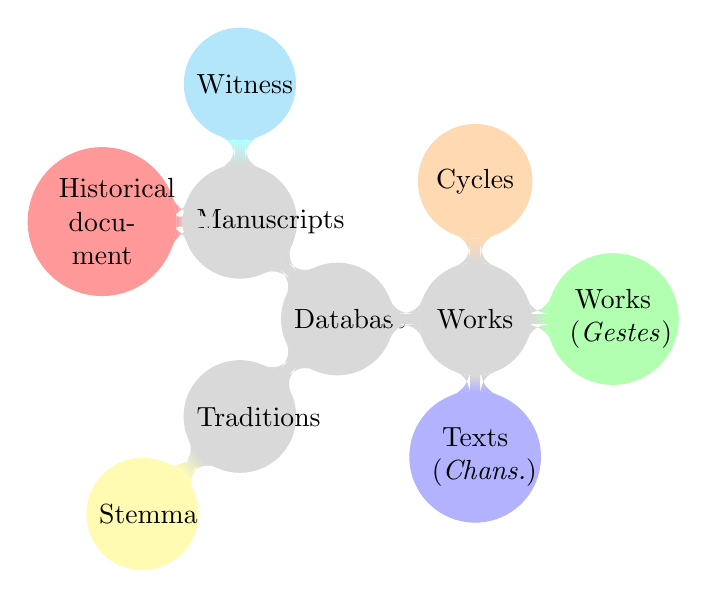
\begin{tikzpicture}[grow cyclic, text width=1.1cm, align=flush center, every node/.style=concept, concept color=gray!30,
        level 1/.style={level distance=1.75cm,sibling angle=135},
        level 2/.style={level distance=1.75cm,sibling angle=90}]
        
        \node{{Database}}
            child [concept color=gray!30] { node{Traditions}
                child [concept color=yellow!30] {node{Stemma}}
            }
            child [concept color=gray!30] { node{Works}
                child [concept color=blue!30] {node{Texts (\textit{Chans.})}}
                child [concept color=green!30] {node{Works (\textit{Gestes})}}
                child [concept color=orange!30] {node{Cycles}}
            }
            child [concept color=gray!30] { node{Manuscripts}
                child [concept color=cyan!30] {node{Witness}}
                child [concept color=red!40] {node{Historical document}}
            }
        ;
    \end{tikzpicture}
    
\end{frame}

\section{Entities}
\tikzstyle{arrow} = [thick,->,>=stealth]
    \tikzstyle{cycle} = [
        rectangle,
        minimum width=1.5cm,
        minimum height=1cm,
        text width=1.5cm,
        text centered,
        draw=black,
        fill=orange!30
    ]
    \tikzstyle{geste} = [
        rectangle,
        minimum width=1.5cm,
        minimum height=1cm,
        text width=1.5cm,
        text centered,
        draw=black,
        fill=green!30
    ]
    \tikzstyle{chanson} = [
        rectangle,
        minimum width=1.5cm,
        minimum height=1cm,
        text width=1.5cm,
        text centered,
        draw=black,
        fill=blue!30
    ]
    \tikzstyle{witness} = [
        rectangle,
        minimum width=1.5cm,
        minimum height=1cm,
        text width=1.5cm,
        text centered,
        draw=black,
        fill=cyan!30
    ]
    \tikzstyle{doc} = [
        rectangle,
        minimum width=2cm,
        minimum height=1cm,
        text width=2cm,
        text centered,
        draw=black,
        fill=red!30
    ]

\begin{frame}
    \frametitle{5 core entities: from abstract to concrete}

    \centering

    \smartdiagramset{
        priority arrow height advance=1.2cm,
        priority arrow head extend=0.18cm,
        priority arrow width=2cm,
        priority tick size=3pt,
        }
    \tikzset{priority arrow/.append style={rotate=180,anchor=0,xshift=10,}}
    \smartdiagram[priority descriptive diagram]{
        \textbf{Historical Document}:\\A physical copy/edition of the instance,
        \textbf{Witness}:\\An instance of the version of a story,
        \textbf{Text [\textit{Chanson}]}:\\A version of the story,
        \textbf{Work [\textit{Geste}]}:\\A story,
        \textbf{Cycle}:\\A collection of stories
    }

\end{frame}


\begin{frame}
    \frametitle{5 core entities: Marvel example 1}

    \centering

    \smartdiagramset{
        priority arrow height advance=1.2cm,
        priority arrow head extend=0.18cm,
        priority arrow width=2cm,
        priority tick size=3pt,
        }
    \tikzset{priority arrow/.append style={rotate=180,anchor=0,xshift=10,}}
    \smartdiagram[priority descriptive diagram]{
        \textbf{Historical Document}:\\A physical copy of issue 39,
        \textbf{Witness (instance of version)}:\\"How Green Was My Goblin!"\text{,} \textit{The Amazing Spider-Man}\text{,} vol. 1\text{,} no. 39 (1966),
        \textbf{Text (version of story)}:\\Green Goblin follows Peter down an alley,
        \textbf{Work (aka "story")}:\\Green Goblin learns of Spider-Man's identity,
        \textbf{Cycle}:\\Spider-Man - Peter Parker
    }
\end{frame}


\begin{frame}
    \frametitle{5 core entities: Marvel example 2}

    \centering

    \smartdiagramset{
        priority arrow height advance=1.2cm,
        priority arrow head extend=0.18cm,
        priority arrow width=2cm,
        priority tick size=3pt,
        }
    \tikzset{priority arrow/.append style={rotate=180,anchor=0,xshift=10,}}
    \smartdiagram[priority descriptive diagram]{
        \textbf{Historical Document}:\\A DVD copy of the film,
        \textbf{Witness (instance of version)}:\\\textit{Spider-Man} (2002)\\Bibliothèque du cinéma François Truffaut - P RAIM,
        \textbf{Text (version of story)}:\\Goblin notices Peter's wound during dinner,
        \textbf{Work (aka "story")}:\\Green Goblin learns of Spider-Man's identity,
        \textbf{Cycle}:\\Spider-Man - Peter Parker
    }
\end{frame}

\begin{frame}
    \frametitle{5 core entities: \textsc{LostMa} example}

    \centering

    \smartdiagramset{
        priority arrow height advance=1.2cm,
        priority arrow head extend=0.18cm,
        priority arrow width=2cm,
        priority tick size=3pt,
        }
    \tikzset{priority arrow/.append style={rotate=180,anchor=0,xshift=10,}}
    \smartdiagram[priority descriptive diagram]{
        \textbf{Historical Document}:\\Folios 1ra-68b of Fr. Z. 4 (=225),
        \textbf{Witness}:\\Manuscript with siglum V$^1$,
        \textbf{Text}:\\The Franco-Italian chanson \textit{Romanus Aspremontis},
        \textbf{Work}:\\The geste \textit{Aspremont},
        \textbf{Cycle}:\\\textit{Charlemagne - Agolant}
    }
        
\end{frame}

\begin{frame}{Parent-children relationships}

    \tiny
    
    \begin{tikzpicture}[node distance=2.25cm]
        \node [cycle] (cycle0) {\textbf{Cycle}: \textit{Charlemagne}};
        \node [cycle, below of=cycle0] (cycle1) {\textbf{Cycle}: \textit{Charlemagne - Agolant}};
        \draw [arrow] (cycle0) -- (cycle1);
        
        \node [geste, right of=cycle1, yshift=-1cm] (work) {\textbf{Work}: \textit{Aspremont}};
        \node [geste, right of=cycle1, yshift=1cm] (work0) {\textbf{Work}: \textit{Agolant}};
        \draw [arrow] (cycle1) -- (work);
        \draw [arrow] (cycle1) -- (work0);

        \node [chanson, right of=work, yshift=-1cm] (text0) {\textbf{Text}: \textit{Aspremont} (Arlima 762)};
        \draw [arrow] (work) -- (text0);

        \node [witness, right of=text0, yshift=3.75cm] (witness0) {\textbf{Witness}:\\Cha};
        \draw [arrow] (text0) -- (witness0);

        \node [chanson, right of=work, yshift=0.5cm] (text1) {\textbf{Text}: \textit{Apremonte} (Arlima 761)};
        \draw [arrow] (work) -- (text1);

        \node [witness, right of=text0, yshift=2.25cm] (witness4) {\textbf{Witness}:\\Trento};
        \node [witness, right of=text0, yshift=0.75cm] (witness1) {\textbf{Witness}:\\F};
        \node [witness, right of=text0, yshift=-0.75cm] (witness2) {\textbf{Witness}:\\V$^1$};
        \node [witness, right of=text0, yshift=-2.25cm] (witness3) {\textbf{Witness}:\\V$^2$};
        \draw [arrow] (text0) -- (witness4);
        \draw [arrow] (text0) -- (witness1);
        \draw [arrow] (text0) -- (witness2);
        \draw [arrow] (text0) -- (witness3);

        \node [doc, right of=witness0] (doc0) {\textbf{Document}:\\Chantilly\text{,} Bibl. du Château\text{,} 470};
        \node [doc, right of=witness1] (doc1) {\textbf{Document}:\\Firenze\text{,} Bibl. nazionale centrale\text{,} Magl. cl. VII\text{,} 932};
        \node [doc, right of=witness4] (doc4) {\textbf{Document}:\\Trento\text{,} Bibl. di San Bernardino\text{,} Arch. 320};
        \node [doc, right of=witness2] (doc2) {\textbf{Document}:\\Venezia\text{,}Bibl. nazionale Marciana\text{,} Fr. Z. 4\text{,} f. 1ra-68b};
        \node [doc, right of=witness3] (doc3) {\textbf{Document}:\\Venezia\text{,}Bibl. nazionale Marciana\text{,} Fr. Z. 6(=226)\text{,} f. 6r-69r};
        \draw [arrow] (witness0) -- (doc0);
        \draw [arrow] (witness1) -- (doc1);
        \draw [arrow] (witness2) -- (doc2);
        \draw [arrow] (witness3) -- (doc3);
        \draw [arrow] (witness4) -- (doc4);

    \end{tikzpicture}

\end{frame}



\section{Entity Relationships}
\tikzstyle{arrow} = [thick,->,>=stealth]
    \tikzstyle{cycle} = [
        rectangle,
        minimum width=3cm,
        minimum height=1cm,
        text width=3cm,
        text centered,
        draw=black,
        fill=orange!30
    ]
    \tikzstyle{geste} = [
        rectangle,
        minimum width=3cm,
        minimum height=1cm,
        text width=3cm,
        text centered,
        draw=black,
        fill=green!30
    ]
    \tikzstyle{chanson} = [
        rectangle,
        minimum width=3cm,
        minimum height=1cm,
        text width=3cm,
        text centered,
        draw=black,
        fill=blue!30
    ]
    \tikzstyle{witness} = [
        rectangle,
        minimum width=3cm,
        minimum height=1cm,
        text width=3cm,
        text centered,
        draw=black,
        fill=cyan!30
    ]
    \tikzstyle{doc} = [
        rectangle,
        minimum width=3cm,
        minimum height=1cm,
        text width=3cm,
        text centered,
        draw=black,
        fill=red!30
    ]

\begin{frame}{Inter-entity relationships}

    \centering
    
    \begin{tikzpicture}[node distance=1.66cm]
        \node[doc] (document) {\textbf{Document}};
        \node[witness, below of=document] (witness) {\textbf{Witness}};
        \node[chanson, below of=witness] (chanson) {\textbf{Text}};
        \node[geste, below of=chanson] (geste) {\textbf{Work}};
        \node[cycle, below of=geste] (cycle) {\textbf{Cycle}};

        \draw[arrow] (geste) -- (cycle) node[midway, right] {is grouped within};
        \draw[arrow] (chanson) -- (geste) node[midway, right] {is a story from};
        \draw[arrow] (witness) -- (chanson) node[midway, right]{is an instance of};
        \draw[arrow] (document) -- (witness) node[midway, right]{contains};
    \end{tikzpicture}

\end{frame}

\begin{frame}{Cycle-to-cycle relationships}

    A cycle can be related to another cycle.

    \begin{center}
    \begin{tikzpicture}[node distance=7cm]
        \node [cycle] (cycle1) {\textbf{Cycle}:\\Charlemagne};
        \node [cycle, right of=cycle1] (cycle2) {\textbf{Cycle}:\\Charlemagne - Agolant};
        \draw [arrow] (cycle2) -- (cycle1) node[midway, below]{IsGroupedWithin};
    \end{tikzpicture}
    \end{center}

    
\end{frame}

\begin{frame}{Text-to-text relationships}

    A text can be derivative of / related to another text in multiple ways.

    \begin{center}
    \begin{tikzpicture}[node distance=2cm]
        \node [chanson] (text1) {\textbf{Text}:\\\textit{Aspramonte}};
        \node [chanson, right of=text1, xshift=5cm] (text2) {\textbf{Text}:\\\textit{Aspremont}};
        \draw [arrow] (text1) -- (text2) node[midway, below]{IsATranslationOf};
        \node [geste, above of=text1, xshift=3.5cm] (geste) {\textbf{Work}:\\\textit{Aspremont}};
        \draw [arrow] (text1) -- (geste) node[midway, left]{IsAStoryFrom};
        \draw [arrow] (text2) -- (geste) node[midway, right]{IsAStoryFrom};
    \end{tikzpicture}
    \end{center}

    \vspace{1em}
    Text A is \ldots Text B:

    \begin{itemize}
        \item is a \textit{version} of [inverse: is a \textit{model} for]
        \item is a \textit{translation} of
        \item is a \textit{prosification} of [inverse: is a \textit{reversification} of]
        \item is an \textit{abridgement} of [inverse: is an \textit{amplification} of]
    \end{itemize}

    \vspace{1em}
    
\end{frame}

\end{document}
